\documentclass{standalone}
\usepackage{tikz}
\usepackage{pgfplots}
\pgfplotsset{compat=newest}
\usepackage{pgfmath}
\usepackage{tikz-cd}
\usepackage{pgffor}
\usepackage{tkz-euclide}
\usetkzobj{all}
\usepgfplotslibrary{fillbetween}
\usetikzlibrary{
	calc,
	angles,
	quotes,
	arrows.meta,
	decorations.markings,
	math,
	backgrounds,
	pgfplots.statistics,
	matrix,
	patterns,
	shapes.geometric,
	spy,
	intersections,
}
\begin{document}
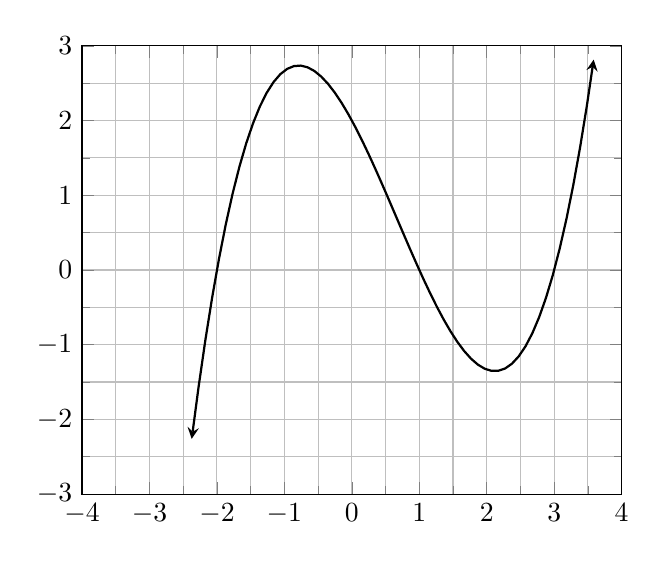
\begin{tikzpicture}[scale=1]
\begin{axis}[
  grid=both,
  ymin=-3,
  ymax=3,
  xmax=4,
  xmin=-4,
  xtick={-4,-3,-2,...,3,4},
  ytick={-4,-3,-2,...,3,4},
  minor tick num=1,
]
 \addplot[thick, samples=100, restrict y to domain=-2.9:2.9, name path=A, stealth-stealth]   {1/3*(x+2)*(x-1)*(x-3)};
% \addplot[thick, draw, -stealth] (0.95, 1.92)--(-3.3,-3.3);
  % \node[draw,shape=circle, minimum size=2mm,inner sep=0pt,outer sep=0pt, fill=black] at (2,-1) {};
  % \node[draw,shape=circle, minimum size=2mm,inner sep=0pt,outer sep=0pt] at (1,-2) {};
  % \node[draw,shape=circle, minimum size=2mm,inner sep=0pt,outer sep=0pt, fill=black] at (1,2) {};
\end{axis}
\end{tikzpicture}
\end{document}